\section{Computing Forces with FFT}

\lstinputlisting[caption={Code for the Cloud-In-Cell method to distribute densities on the grid.}]{cic.py}
\lstinputlisting[caption={All code to apply the procedures outlined below to compute the potential.}]{fourier.py}
\lstinputlisting[caption={Implementation of the recursive Cooley-Tukey algorithm with trigonometric recurrence.}, linerange={120-195}]{algorithms.py}

In the previous section we could brute force the computation of the motion of the planets relatively easy because there are only eight objects, and eight relevant forces. However if interparticle interactions were important this task would have already been a lot more difficult as there would have been 56 forces to be taken into account at each timestep. Expanding beyond $N = 8$ rapidly worsens this problem. In this section we will investigate one of the methods to transform such a problem from $\mathcal{O}(N^2)$ to $\mathcal{O}(N\log(N))$, namely the Fast Fourier Transform (FFT). We will test this by computing the gravitational potential on a grid for a volume of 16x16x16 units with 1024 particles, each with a mass of 1. The edges of the grid are connected such taht $x = 16 \equiv 0$. The mass of each particle is assigned to a grid point using the Cloud-In-Cell method written by Zorry Belcheva, given above. We start by filling out the grid, and present the density contrast $\delta = (\rho-\overline{\rho})/\overline{\rho}$ at 4 separate 2D slices at constant z Figure

\begin{figure}
    \centering
    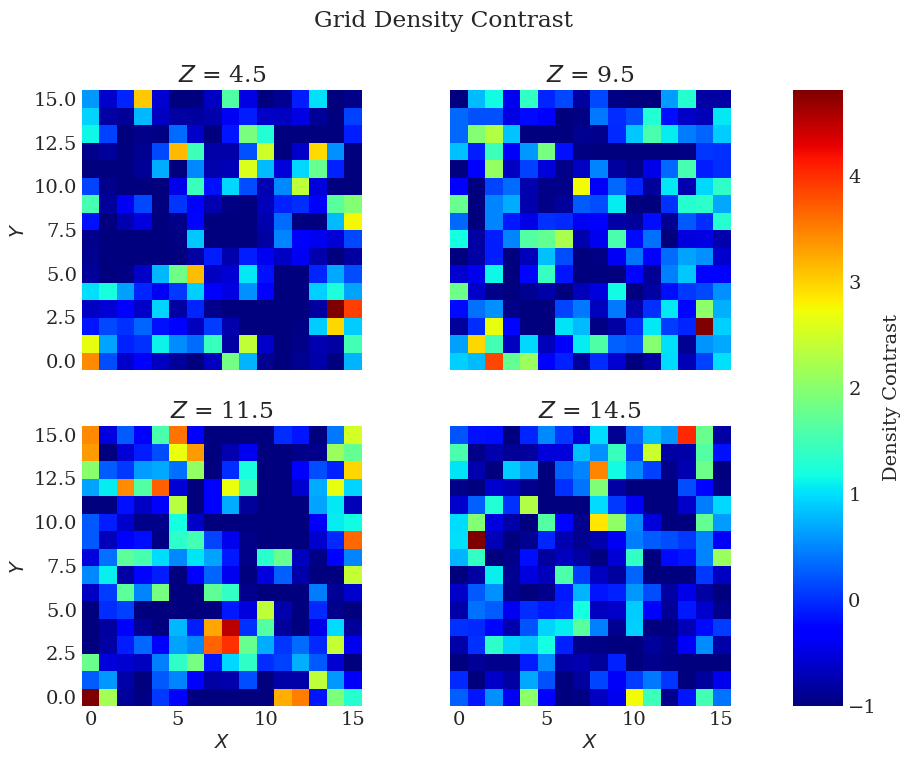
\includegraphics[width=0.8\textwidth]{results/density_contrast_slices}
    \caption{Density contrast $\delta$ in four separate 2D slices at constant z computed using the Cloud-In-Cell method on a 3D grid.}
    \label{fig:dens_contrast}
\end{figure}

To calculate the gravitational force, we first need the gravitational potential which we can compute using the Poisson equation

\begin{equation}
    \nabla^2 \Phi = 4\pi G\rho = 4\pi G\, \overline\rho(1 + \delta)
\end{equation}

We can simplify this because we only need to solve the spatial dependence of this equation, i.e. $\nabla^2\Phi \propto \delta$. Using fourier transforms we can easily do this with by computing the foruier transform of the density contrast, using that to compute the transformed potential, and then applying an inverse fourier transformation to find the true potential. Mathematically, we can write this as

\begin{align*}
    \delta & \xrightarrow{\mathrm{FFT}} \tilde{\delta} \propto k^2\tilde{\Phi} \\
    \tilde{\Phi} & \propto \frac{\tilde{\delta}}{k^2} \\
    \frac{\tilde{\delta}}{k^2} & \xrightarrow{\mathrm{IFFT}} \Phi
\end{align*}

The only question that now remains is what $k$ is. We can calculate this from the wavenumber vector as

\begin{equation}
    k^2 = k_x^2 + k_y^2 + k_z^2.
\end{equation}

Where $k_x$, $k_y$, and $k_z$ are just equal to the grid coordinates and therefore take on integer values from $0$ to $15$. 

The FFT algorithm in this work is implemented using the recursive Cooley-Tukey algorithm with trigonometric recurrence for additional speed up. 

\subsection{Results}

We start with the first two steps from our potential calcuation procedure, i.e. apply a fourier transform to the density contrast, and divide it by $k^2$. In Figure \ref{fig:fft_potential} we present the log of the absolute value of $\tilde\Phi$. We take the absolute value because there is a complex component which we want to include in the figure. 

\begin{figure}
    \centering
    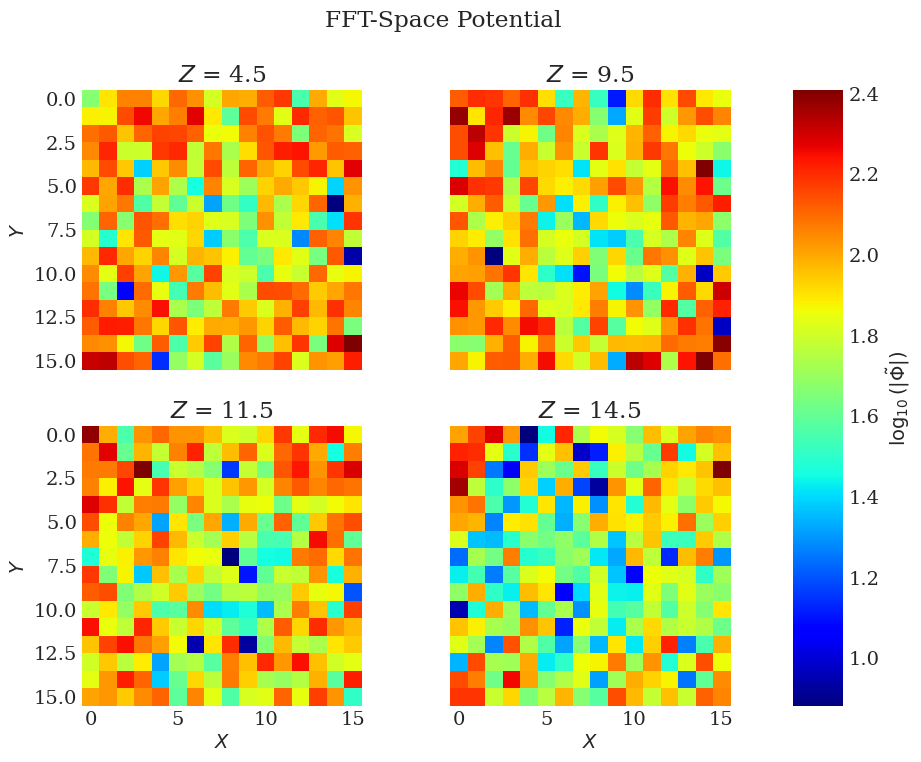
\includegraphics[width=0.8\textwidth]{results/fft_potential.png}
    \caption{Logarithm of the absolute value of the fourier transformed gravitational potential, this is equal to the fourier transformed density contrast divided by $k^2$.}
    \label{fig:fft_potential}
\end{figure}

We then apply the inverse Fourier Transform with the FFT algorithm to the data shown in Figure \ref{fig:fft_potential} to find the gravitational potential which we present in Figure \ref{fig:potential}.

\begin{figure}
    \centering
    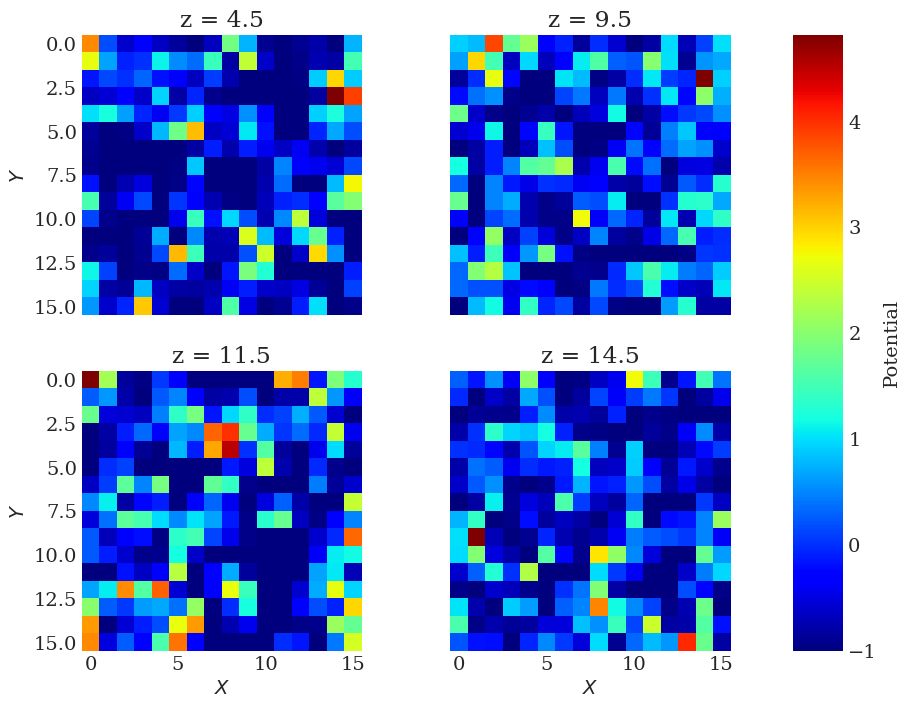
\includegraphics[width=0.8\textwidth]{results/potential_slices.png}    
    \caption{Gravitational potential of the density contrast grid shown in Fiugre \ref{fig:dens_contrast}, computed using fourier transformations as described in text.}
    \label{fig:potential}
\end{figure}

We can see that the calculated potentials are quite smooth when compared to the more eratic distritubution of mass in Figure \ref{fig:dens_contrast}. However this makes sense as we can see from the Poisson equation that the density contrast influences only the second order derivative of the potential. Comparing the density contrast and potential figures, we can see that the regions of high and low density correspond well to the regions of high and low potential respectively, which ofcourse is exactly as expected for the gravitational potential. For example the low density region in the center of the $Z = 4.5$ slice corresponds to a potential well, and the high density 'square' in the $Z = 11.5$ slice at $Y = 3$ corresponds to a high potential arm reaching towards the center. 

As a final note, a test run of the procedure outlined above with $k = 1$ resulted in a 'potential' that was exactly equal to the density contrast. While not physically relevant, this is a proof that the FFT algorithms properly worked because the inverse fourier transform of a fourier transformed dataset should be equal to the original data set.
